A revisão bibliográfica, também chamada de revisão da literatura ou fundamentação teórica, é uma etapa fundamental de qualquer trabalho acadêmico. Seu objetivo é situar a pesquisa no contexto do conhecimento existente, identificando lacunas, tendências e contribuições anteriores.

\section{Propósito da Revisão Bibliográfica}

A revisão bibliográfica cumpre múltiplos propósitos:

\begin{enumerate}
    \item demonstrar domínio sobre o tema de pesquisa;
    \item identificar o estado da arte e as lacunas existentes;
    \item justificar a relevância e originalidade do trabalho;
    \item estabelecer a base teórica para a metodologia adotada; e
    \item evitar duplicação de esforços já realizados.
\end{enumerate}

Recomenda-se que a revisão seja organizada por temas ou conceitos, e não simplesmente por ordem cronológica de publicação. Cada trabalho citado deve ser analisado criticamente, destacando suas contribuições e limitações.

\section{Normas ABNT para Trabalhos Acadêmicos}

A elaboração de dissertações e teses no Brasil é regida por um conjunto de normas da \ac{ABNT}. As principais são:

\begin{enumerate}
    \item NBR 14724 -- Trabalhos acadêmicos: apresentação;
    \item NBR 6023 -- Referências: elaboração;
    \item NBR 10520 -- Citações em documentos;
    \item NBR 6024 -- Numeração progressiva das seções;
    \item NBR 6027 -- Sumário: apresentação;
    \item NBR 6028 -- Resumo: apresentação; e
    \item NBR 6034 -- Índice: apresentação.
\end{enumerate}

Este template implementa automaticamente a maioria dessas normas através da classe \texttt{ita.cls} e do pacote Bib\LaTeX{} com estilo ABNT.

\section{Tipos de Citação}

O sistema Bib\LaTeX{} com estilo ABNT oferece diversos comandos para citação. A seguir, demonstramos os principais tipos.

\subsection{Citação Indireta}

A citação indireta ocorre quando parafraseamos as ideias de um autor. Utiliza-se o comando \texttt{\textbackslash cite\{\}}:

\begin{itemize}
    \item Segundo a literatura, sistemas de controle robusto são essenciais para aplicações críticas \cite{Sbornian2004}.
    \item Diversos autores trataram do tema \cite{Sbornian2004, Joea2003}.
\end{itemize}

\subsection{Citação com Autor no Texto}

Quando o nome do autor faz parte da sentença, utiliza-se \texttt{\textbackslash textcite\{\}}:

\begin{itemize}
    \item \textcite{Nascimento1970} apresentou os fundamentos teóricos do problema.
    \item Conforme demonstrado por \textcite{Sbornian2004}, a abordagem é viável.
\end{itemize}

\subsection{Citação Direta}

Citações diretas curtas (até 3 linhas) são inseridas no texto entre aspas. Para citações longas, utiliza-se o ambiente \texttt{quote} ou \texttt{citacao}:

\begin{quote}
``A formatação adequada de um trabalho acadêmico contribui para sua clareza e credibilidade, facilitando a comunicação científica.''
\end{quote}

\section{Elementos de Apoio}

A revisão bibliográfica frequentemente utiliza tabelas e equações para sintetizar informações. A Tabela \ref{tab:exemplo} demonstra a formatação adequada.

\begin{table}[ht]
\caption{Comparativo entre abordagens metodológicas}
\label{tab:exemplo}
\centering
\begin{tabular}{lccc}
    \hline
    Abordagem & Complexidade & Precisão & Custo \\
    \hline
    Analítica & Baixa & Alta & Baixo \\
    Numérica & Média & Média & Médio \\
    Experimental & Alta & Variável & Alto \\
    \hline
\end{tabular}
\end{table}

Equações também são frequentes em revisões de áreas técnicas. Por exemplo, a equação de Lagrange é fundamental em mecânica analítica:

\begin{equation} \label{eq:lagrange}
\frac{d}{dt}\left(\frac{\partial L}{\partial \dot{q}}\right) - \frac{\partial L}{\partial q} = \tau
\end{equation}

\noindent onde $L = T - V$ representa o Lagrangiano do sistema, $T$ a energia cinética, $V$ a energia potencial, $q$ as coordenadas generalizadas e $\tau$ as forças generalizadas.

\section{Figuras Vetoriais com PGFPlots}

O pacote PGFPlots permite criar gráficos de alta qualidade diretamente em \LaTeX{}, com vantagens significativas sobre imagens externas:

\begin{enumerate}
    \item qualidade vetorial (sem pixelização em qualquer escala);
    \item consistência tipográfica (mesma fonte do documento);
    \item facilidade de edição (dados no próprio código); e
    \item arquivos leves e versionáveis.
\end{enumerate}

A Figura \ref{fig:linha} apresenta um exemplo de gráfico de linhas comparando dados experimentais com modelo teórico.

\begin{figure}[ht]
\centering
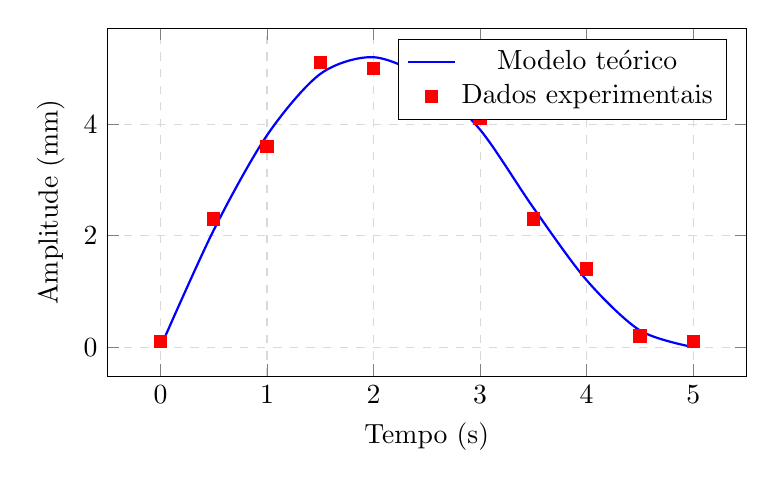
\begin{tikzpicture}
\begin{axis}[
    width=0.8\textwidth,
    height=6cm,
    xlabel={Tempo (s)},
    ylabel={Amplitude (mm)},
    legend pos=north east,
    grid=major,
    grid style={dashed,gray!30},
]
\addplot[blue, thick, mark=none, smooth] coordinates {
    (0,0) (0.5,2.1) (1,3.8) (1.5,4.9) (2,5.2) (2.5,4.8) (3,3.9) (3.5,2.5) (4,1.2) (4.5,0.3) (5,0)
};
\addlegendentry{Modelo teórico}

\addplot[red, thick, only marks, mark=square*] coordinates {
    (0,0.1) (0.5,2.3) (1,3.6) (1.5,5.1) (2,5.0) (2.5,4.6) (3,4.1) (3.5,2.3) (4,1.4) (4.5,0.2) (5,0.1)
};
\addlegendentry{Dados experimentais}
\end{axis}
\end{tikzpicture}
\caption{Comparação entre modelo teórico e dados experimentais.}
\label{fig:linha}
\end{figure}

Para comparações categóricas, gráficos de barras são frequentemente utilizados, como ilustrado na Figura \ref{fig:barras}.

\begin{figure}[ht]
\centering
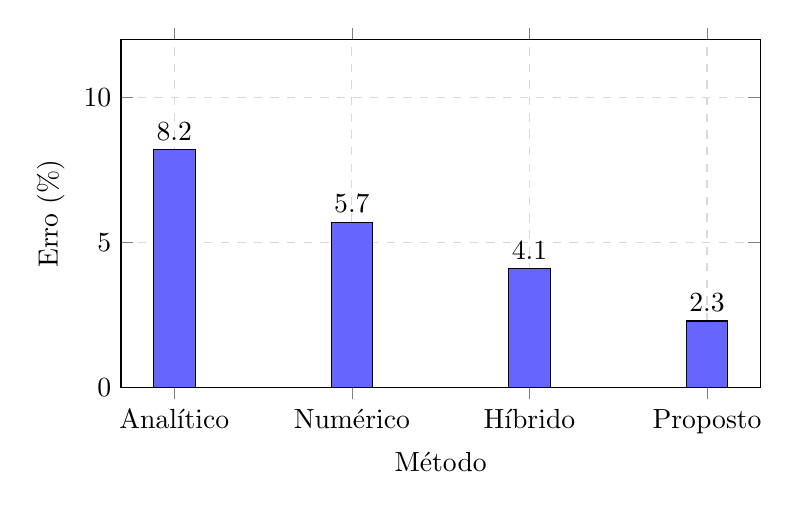
\begin{tikzpicture}
\begin{axis}[
    width=0.8\textwidth,
    height=6cm,
    ybar,
    bar width=15pt,
    xlabel={Método},
    ylabel={Erro (\%)},
    symbolic x coords={Analítico, Numérico, Híbrido, Proposto},
    xtick=data,
    nodes near coords,
    nodes near coords align={vertical},
    ymin=0,
    ymax=12,
    grid=major,
    grid style={dashed,gray!30},
    ymajorgrids=true,
]
\addplot[fill=blue!60] coordinates {
    (Analítico,8.2) (Numérico,5.7) (Híbrido,4.1) (Proposto,2.3)
};
\end{axis}
\end{tikzpicture}
\caption{Comparativo de erro entre diferentes métodos.}
\label{fig:barras}
\end{figure}

\section{Boas Práticas}

Ao redigir a revisão bibliográfica, recomenda-se:

\begin{enumerate}
    \item utilizar fontes primárias sempre que possível;
    \item priorizar publicações recentes e de periódicos com revisão por pares;
    \item manter consistência na forma de citação ao longo do texto;
    \item evitar citações excessivas em uma única sentença; e
    \item conectar os trabalhos citados com a proposta da pesquisa.
\end{enumerate}
